\documentclass{article}

\usepackage{pandekten}
\usepackage{dashrule}

\makeatletter
\newcommand*{\shifttext}[1]{%
  \settowidth{\@tempdima}{#1}%
  \hspace{-\@tempdima}#1%
}
\newcommand{\plabel}[1]{%
\shifttext{\textbf{#1}\quad}%
}
\newcommand{\prule}{%
\begin{center}%
\hdashrule[0.5ex]{.99\linewidth}{1pt}{1pt 2.5pt}%
\end{center}%
}

\makeatother

\setlength{\parindent}{0pt}

\title{Assignment 1}
\author{Ze Chen}

\begin{document}

\maketitle

\plabel{1 (1a)}%
A primitive cell and a Wigner-Seitz cell are shown as the shaded region on the left and right, respectively.
\begin{center}
    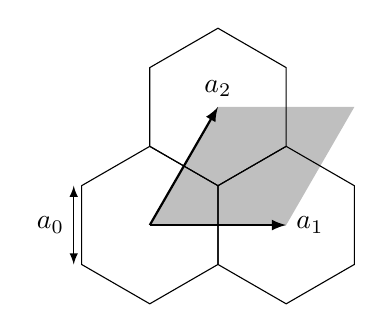
\begin{tikzpicture}
        \draw[draw=none,fill=lightgray] (210:1) -- (-30:1) --(30:2) -- (90:1) -- cycle;
        \draw (0,0) --++ (30:1) --++(90:1) --++(150:1) --++(210:1) --++(270:1) -- cycle;
        \draw (0,0) --++ (150:1) --++(210:1) --++(270:1) --++(330:1) --++(30:1) -- cycle;
        \draw (0,0) --++ (270:1) --++(330:1) --++(30:1) --++(90:1) --++(150:1) -- cycle;
        \draw[thick,-latex] (210:1) -- (-30:1) node[right] {$\vb{a}_1$};
        \draw[thick,-latex] (210:1) -- (90:1) node[above] {$\vb{a}_2$};
        \draw[latex-latex] (-0.1,0) ++ (150:1) ++(210:1) --++(270:1) node[midway,left] {$a_0$};
    \end{tikzpicture}
    \hspace{2cm}
    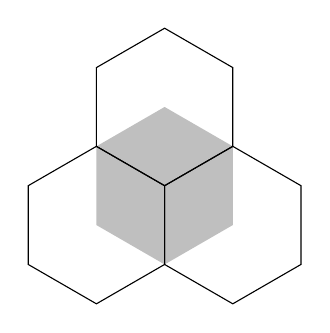
\begin{tikzpicture}
        \draw[draw=none,fill=lightgray] (30:1) --++ (-90:1) --++ (-150:1) --++ (-210:1) --++ (-270:1) --++ (-330:1) -- cycle;
        \draw (0,0) --++ (30:1) --++(90:1) --++(150:1) --++(210:1) --++(270:1) -- cycle;
        \draw (0,0) --++ (150:1) --++(210:1) --++(270:1) --++(330:1) --++(30:1) -- cycle;
        \draw (0,0) --++ (270:1) --++(330:1) --++(30:1) --++(90:1) --++(150:1) -- cycle;
    \end{tikzpicture}
\end{center}
The coordinates of primitive vectors are given by
\[ \vb{a}_1 = \qty(\sqrt{3}a_0, 0)^\intercal = \begin{pmatrix} \SI{0.246}{\nano\meter} \\ 0 \end{pmatrix},\quad \vb{a}_2 = \qty(\frac{\sqrt{3}}{2}a_0,\frac{3}{2}a_0)^\intercal = \begin{pmatrix}\SI{0.123}{\nano\meter} \\ \SI{0.213}{\nano\meter}\end{pmatrix}. \]

\plabel{(1b)}%
Two.

\plabel{(1c)}%
The components are given by (with reciprocal vectors as row vectors)
\[ \begin{pmatrix}
    \vb{b}_1 \\
    \vb{b}_2
\end{pmatrix} = 2\pi \begin{pmatrix}
    \vb{a}_1 & \vb{a}_2
\end{pmatrix}^{-1} = \frac{2\pi}{a_0} \begin{pmatrix}
    \sqrt{3}/3 & -1/3 \\
    0 & 2/3
\end{pmatrix} = \begin{pmatrix}
    \SI{25.55}{\per\nano\meter} & \SI{-14.75}{\per\nano\meter} \\
    \num{0} & \SI{29.50}{\per\nano\meter} \\
\end{pmatrix}. \]
The Wigner-Seitz Brillouin zone is shown as the shaded region.
\begin{center}
    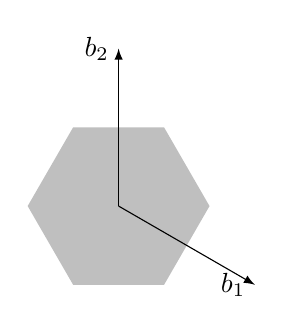
\begin{tikzpicture}
        \draw[draw=none,fill=lightgray] ({sqrt(3)/3},1) -- (-{sqrt(3)/3},1) -- ({-2/sqrt(3)},0) -- (-{sqrt(3)/3},-1) -- ({sqrt(3)/3},-1) -- ({2/sqrt(3)},0) -- cycle;
        \draw[-latex] (0,0) -- (-30:2) node[left] {$\vb{b}_1$};
        \draw[-latex] (0,0) -- (90:2) node[left] {$\vb{b}_2$};
    \end{tikzpicture}
\end{center}

\plabel{(2a)}%
The Wigner-Seitz cell is shown below.
\begin{center}
    \includegraphics[width=6cm]{img/1.2a.WS/main.pdf}
\end{center}

\plabel{(2b)}%
The reciprocal primitive vectors are given by
\[ \begin{pmatrix}
    \vb{b}_1 \\
    \vb{b}_2
\end{pmatrix} = 2\pi \begin{pmatrix}
    \vb{a}_1 & \vb{a}_2
\end{pmatrix}^{-1} = 2\pi \begin{pmatrix}
    1/3 & -1/6 \\
    0 & 1/2
\end{pmatrix}. \]
The reciprocal Wigner-Seitz cell is shown below.
\begin{center}
    \includegraphics[width=6cm]{img/1.2a.BZWS/main.pdf}
\end{center}

\plabel{(3a)}%
The diamond lattice consists of two FCC lattices related by a translation.
It suffices to write down the basis vectors for one of them.
\begin{align*}
    \vb{a}_1 &= (0,a_0/2,a_0/2)^\intercal, \\
    \vb{a}_2 &= (a_0/2,0,a_0/2)^\intercal, \\ 
    \vb{a}_3 &= (a_0/2,a_0/2,0)^\intercal.
\end{align*}

\plabel{(3b)}%
Number of atoms in each primitive cell is given by
\[ N = 8\times \frac{a_0^3}{\det \begin{pmatrix}
    \vb{a}_1 & \vb{a}_2 & \vb{a}_3
\end{pmatrix}} = 2. \]

\plabel{(2c)}%
The reciprocal primitive vectors are given by
\[ \begin{pmatrix}
    \vb{b}_1 \\
    \vb{b}_2 \\
    \vb{b}_3
\end{pmatrix} = 2\pi \begin{pmatrix}
    \vb{a}_1 & \vb{a}_2 & \vb{a}_3
\end{pmatrix}^{-1} = \frac{2\pi}{a_0} \begin{pmatrix}
    -1 & 1 & 1 \\
    1 & -1 & 1 \\
    1 & 1 & -1
\end{pmatrix}. \]

\prule
\plabel{2 (1)}%
We find (for $0\le m < N$)
\[ \frac{1}{N} \sum_{n=0}^{N-1} e^{2\pi i m n / N} = \begin{cases}
    \displaystyle\frac{1 - e^{2\pi i m N/N}}{1 - e^{2\pi i m}} = 0, & \text{if $e^{2\pi i m} \neq 1$}, \\
    1, &\text{otherwise}.
\end{cases} = \delta_{m,0}. \]

\plabel{(2a)}%
With the new canonical pairs $(P,U)$ and $(p,u)$ defined by
\[ P = p_1 + p_2,\quad p = \frac{p_2 - p_1}{2},\quad U = \frac{u_1 + u_2}{2}, \quad u = u_2 - u_1, \]
the Hamiltonian becomes
\[ H = \frac{P^2}{2\cdot 2M} + \frac{p^2}{2\cdot M/2} + \frac{K}{2} u^2, \]
whence we find
\[ \omega_1 = \sqrt{\frac{2K}{M}}. \]

\plabel{(2b)}%
Let
\begin{equation}
    \label{eq:n}
    L = \begin{pmatrix}
        -1 & -1 & & & \\
        -1 & 0 & -1 & & \\
        & -1 & \ddot & \ddot & \\
        & & \ddot & 0 & -1 \\
        & & & -1 & -1
    \end{pmatrix}_{N\times N}.
\end{equation}
We could easily verify the identity
\[ \sum_{n=1}^N L_{n',n} f_{k,n} = -2 \cos\qty(k a_0) f_{k,n'}. \]
Therefore, $\Set*{\begin{pmatrix}
    f_{k,1} & \cdots f_{k,N}
\end{pmatrix}^\intercal}{k}$
is a set of eigenvectors of $L$, which is orthogonal since $L$ is real-symmetric.
$\begin{pmatrix}
    f_{0,1} & \cdots f_{0,N}
\end{pmatrix}^\intercal$ is clearly normalized.
If $k\neq 0$,
\[ \sum_{n=1}^N f_{k,n}^2 = \sum_{n=1}^N \frac{2}{N}\frac{1 + 2\cos\qty(\pi m (2n-1) / N)}{2} = 1. \]
Therefore, $\Set*{\begin{pmatrix}
    f_{k,1} & \cdots f_{k,N}
\end{pmatrix}^\intercal}{k}$ is orthonormal.

\plabel{(2c)}%
Let $r$ and $s$ stand for $u$ or $p$. Then
\begin{align*}
    [\tilde{r}_k,\tilde{s}_{k'}] &= \sum_{n,n'} f_{k,n} f_{k',n'} [r_n,s_{n'}] \\
    &= \begin{cases}
        \displaystyle\sum_{n} i\hbar f_{k,n} f_{k',n} = i\hbar\delta_{k,k'}, & \text{if } r,s = u,p, \\
        0, & \text{if } r,s = u,u \text{ or } r,s=p,p.
    \end{cases}
\end{align*}

\plabel{(2d)}%
Denote by $f$ the matrix
\[ f = \begin{pmatrix}
    f_{0, 1} & \cdots & f_{(N-1)\pi/(n a_0), 1} \\
    \vdots & \ddots & \vdots \\
    f_{0, N} & \vdots & f_{(N-1)\pi/(n a_0), N}
\end{pmatrix}. \]
by $u$ the column vector
\[ u = \begin{pmatrix}
    u_1 & \cdots & u_n
\end{pmatrix}^\intercal \]
and by $p$ the column vector
\[ p = \begin{pmatrix}
    p_1 & \cdots & p_n
\end{pmatrix}^\intercal. \]
Then (with $L$ defined by \cref{eq:n}, and $\lambda_k = -2\cos(k a_0)$)
\begin{align*}
    H &= \frac{1}{2M} p^\intercal p + \frac{K}{2} u^\intercal(L + 2\cdot\mathbbm{1}) u \\
    &= \frac{1}{2M} p^\intercal f f^\intercal p + \frac{K}{2} u^\intercal f f^\intercal(L + 2\cdot\mathbbm{1}) f f^\intercal u \\
    &= \sum_k \frac{1}{2M} \tilde{p}_k \tilde{p}_k + \frac{K}{2} \sum_k (\lambda_k + 2) \tilde{u}_k \tilde{u}_k \\
    &= \frac{p_1 + \cdots + p_n}{NM} + \sum_{k>0} \qty(\frac{\tilde{p}_k^2}{2M} + \frac{M\omega_k^2}{2}\tilde{u}_k^2),
\end{align*}
where
\[ \omega_k = 2\sqrt{\frac{K}{M}}\abs{\sin \frac{ka_0}{2}}. \]

\prule
\plabel{3 (1)}%
It suffices to prove $U^\dagger(t) a_k U(t) = e^{-i\omega_k t} a_k$, which implies $U^\dagger(t) a^\dagger_{-k} U(t) = e^{i\omega_{-k} t} a^\dagger_{-k}$.
Note that
\[ [H_{\mathrm{ph}}, a_k] = -\hbar \omega_k a_k. \]
Therefore, with the BCH formula,
\[ U^\dagger(t) a_k U(t) = e^{-i \omega_k t} a_k. \]

\plabel{(2)}%
Only the terms with equal number of $a_k$ and $a^\dagger_k$ contributes. With $\omega_k = \omega_{-k}$ we find
\begin{align*}
    &\phantom{{}={}} \bra{\psi} u(t) \ket{\psi} \\ &= \sqrt{\frac{\hbar}{2NM\omega_k}} \cdot \frac{1}{2} \times \\
    &{\phantom{{}={}}} \ev**{\qty[ \frac{\qty(a_k)^m}{\sqrt{m!}} e^{ikx_n} e^{-i\omega_k t}a_k \frac{\qty(a^\dagger_k)^{m+1}}{\sqrt{(m+1)!}} + \frac{\qty(a_k)^{m+1}}{\sqrt{(m+1)!}} e^{-ikx_n} e^{i\omega_k t}a_k^\dagger \frac{\qty(a^\dagger_k)^m}{\sqrt{m!}} ]}{0} \\
    &= \sqrt{\frac{\hbar}{2NM\omega_k}} \cdot \sqrt{m+1} \cos(k x_n - \omega_k t).
\end{align*}

\plabel{(3a)}%
$\qty(a_k^\dagger)^m\ket{0}$ are orthogonal for different $m$. Therefore
\[ \bra{\psi(w)}\ket{\psi(w)} = \frac{1}{\mathcal{N}_w} \sum_{m=0}^\infty \frac{\overline{w}^m w^m}{m! m!} \sqrt{m!}\sqrt{m!} = \frac{e^{\abs{w}^2}}{\mathcal{N}_w} = 1 \Rightarrow \mathcal{N}_w = e^{\abs{w}^2}. \]

\plabel{(3b)}%
Let $Z(w,\overline{w}) = \bra{0} e^{\overline{w}a_k} e^{w a^\dagger_k} \ket{0} = e^{\overline{w}w}$. We find
\begin{align*}
    \bra{\psi(w)}a_k\ket{\psi(w)} &= \frac{1}{\mathcal{N}_w} \pdv{Z(w,\overline{w})}{\overline{w}} = w, \\
    \bra{\psi(w)}a_k^\dagger\ket{\psi(w)} &= \frac{1}{\mathcal{N}_w} \pdv{Z(w,\overline{w})}{w} = \overline{w}.
\end{align*}
Therefore
\begin{align*}
    \bra{\psi(w)}u_n(t)\ket{\psi(w)} &= \sqrt{\frac{\hbar}{2N M\omega_k}} (e^{ikx_n} e^{-i\omega_k t}w + e^{-ikx_n}e^{i\omega_k t}\overline{w}) \\
    &= \sqrt{\frac{\hbar}{2N M\omega_k}} \cdot 2\Re (e^{ikx_n} e^{-i\omega_k t}w).
\end{align*}

\prule
\plabel{4 (1)}%
Since the eigenvalues of $n_k$ is given by $\qty{0,1,2,\cdots}$, each with multiplicity $1$,
\[ \tr(e^{-Aa_k a^\dagger_k}) = \tr(e^{-An_k}) = \sum_{n\in\operatorname{eigval}(n_k)} e^{-An} = \frac{1}{1-e^{-A}}. \]

\plabel{(2)}%
Let $N$ denote the number of lattice points.
\begin{align*}
    Z &= \tr e^{-\beta H_{\mathrm{ph}}} = \tr \bigotimes_k e^{-\beta \hbar\omega_k (a^\dagger_k a_k + 1/2)} = \prod_k \tr e^{-\beta \hbar\omega_k n_k - \beta \hbar\omega_k/2} \\
    &= \prod_k \frac{e^{-\beta\hbar\omega_k/2}}{1-e^{-\beta\hbar\omega_k}} = \prod_k \frac{1}{2\sinh (\beta\hbar\omega_k/2)}. \\
    \langle n_k \rangle &= \tr(\rho n_k) = \frac{-1}{\beta\hbar} \pdv{\ln Z}{\omega_k} - \frac{1}{2} = \frac{1}{e^{\beta\hbar\omega_k} - 1}.
\end{align*}

\plabel{(3)}%
\abovedisplayskip=0pt\abovedisplayshortskip=0pt~\vspace*{-\baselineskip}%
\begin{align*}
    E &= -\pdv{\ln Z}{\beta} = \sum_k \hbar\omega_k \qty(\frac{1}{e^{\beta\hbar\omega_k} - 1} + \frac{1}{2}), \\
    F &= -\beta^{-1}\ln Z = \beta^{-1} \sum_k \ln \qty[2 \sinh(\beta\hbar\omega_k/2)], \\
    S = k_{\mathrm{B}}\beta(E - F) &= k_{\mathrm{B}}\sum_k \qty(\frac{\beta\hbar\omega_k}{e^{\beta\hbar\omega_k} - 1} - \ln\qty(1-e^{-\beta\hbar\omega_k})).
\end{align*}

% \bibliographystyle{plain}
% \bibliography{main}

\end{document}
